\chapter[SID]{SID}
\section{Visão Geral}
O SID está estruturado em duas possíveis vertentes, o WEB e o mobile, ele foi
desenvolvido com o objetivo de oferecer uma forma mais intuitiva, dinâmica e amigável
para o administrador e para o telespectador.

Necessitando sempre do uso da rede para realizar atualizações, o SID está dividido
em três módulos, o primeiro deles é o administrador, onde é possível fazer o gerenciamento
completo do conteúdo que será apresentado no segundo modulo, no caso o módulo cliente,
nesse segundo módulo será apresentado as informações que foram cadastradas no módulo
administrador e serão propagadas por monitores ou celulares. O terceiro módulo não é
acessível, ele é encarregado de fazer toda recuperação dos dados que será apresentada na
vertente WEB e mobile

\section{Modulo Administrador}
 \begin{enumerate}
   \item Legenda: 
   \item Texto: 
   \item Data de Início:
   \item Data de Término:
   \item Imagem:
 \end{enumerate}
 
 \begin{figure}[!htb]
\centering
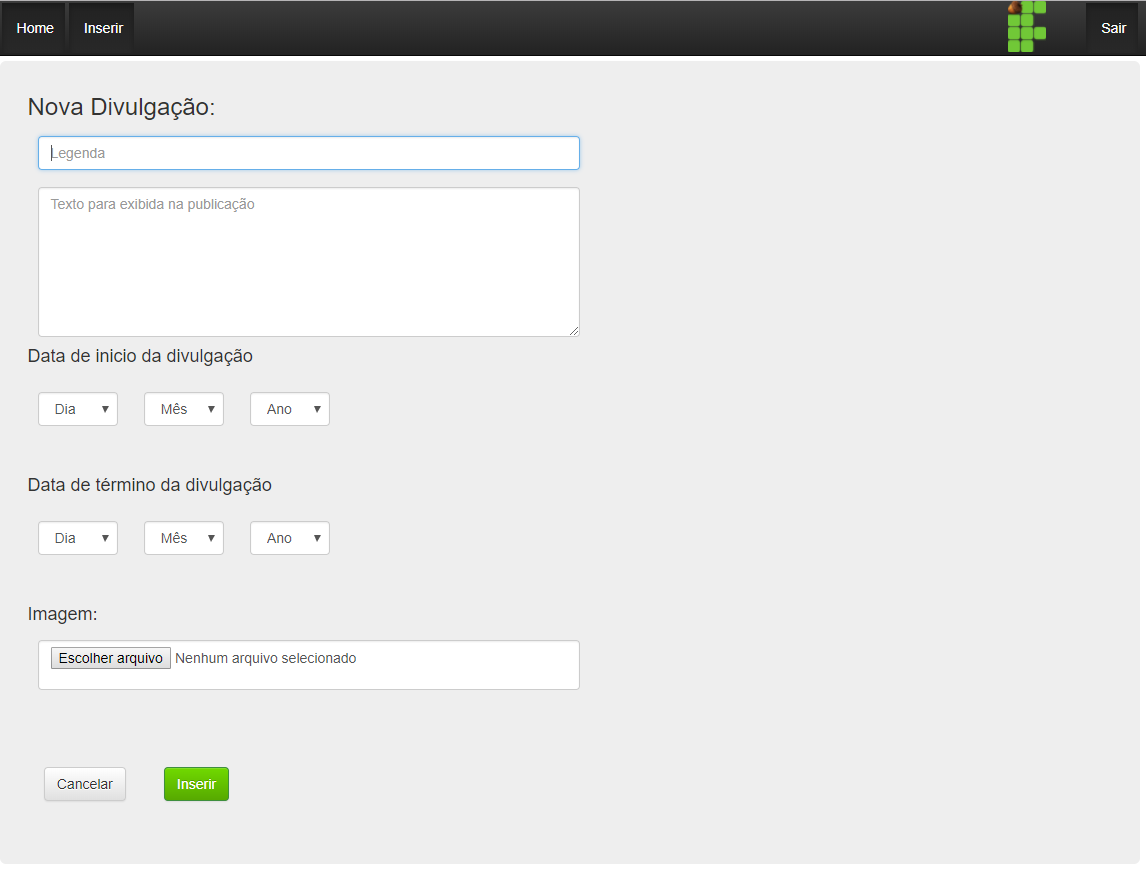
\includegraphics[scale=0.6]{figuras/administrador1}
\caption{Página de inserção no módulo administrador.}
\label{Rotulo}
\end{figure}

\section{Modulo Cliente}
\section{Modulo API}
\section{Arquitetura}
\section{Banco de Dados - Postgres}
\section{Possível solução para Implementação - Rapberry}